\documentclass[12pt, a4paper, titlepage, oneside]{book}
\usepackage[utf8]{inputenc}
\usepackage[italian]{babel} %set language = italian
\usepackage{pdfpages} %include function for pdf
\usepackage{mathptmx} %set font type = times 
\textheight24cm\topmargin0mm\headheight0mm\headsep6mm\oddsidemargin20pt\evensidemargin30pt %margin 
\linespread{1.2} %interlinea
\pagestyle{plain}
\usepackage[backend=biber,style=numeric,sorting=none]{biblatex} %bibliography
\usepackage{csquotes}
\addbibresource{bibliography.bib}

\usepackage{titlesec} %style chapter
\titleformat{\chapter}
  {\normalfont\LARGE\bfseries}{\thechapter}{1em}{}
\titlespacing*{\chapter}{0pt}{3.5ex plus 1ex minus .2ex}{2.3ex plus .2ex}

\usepackage{graphicx} %insert image
\graphicspath{ {./images/} }
\usepackage{wrapfig} %for wrap figures

\usepackage{listings} %for code format


\begin{document}
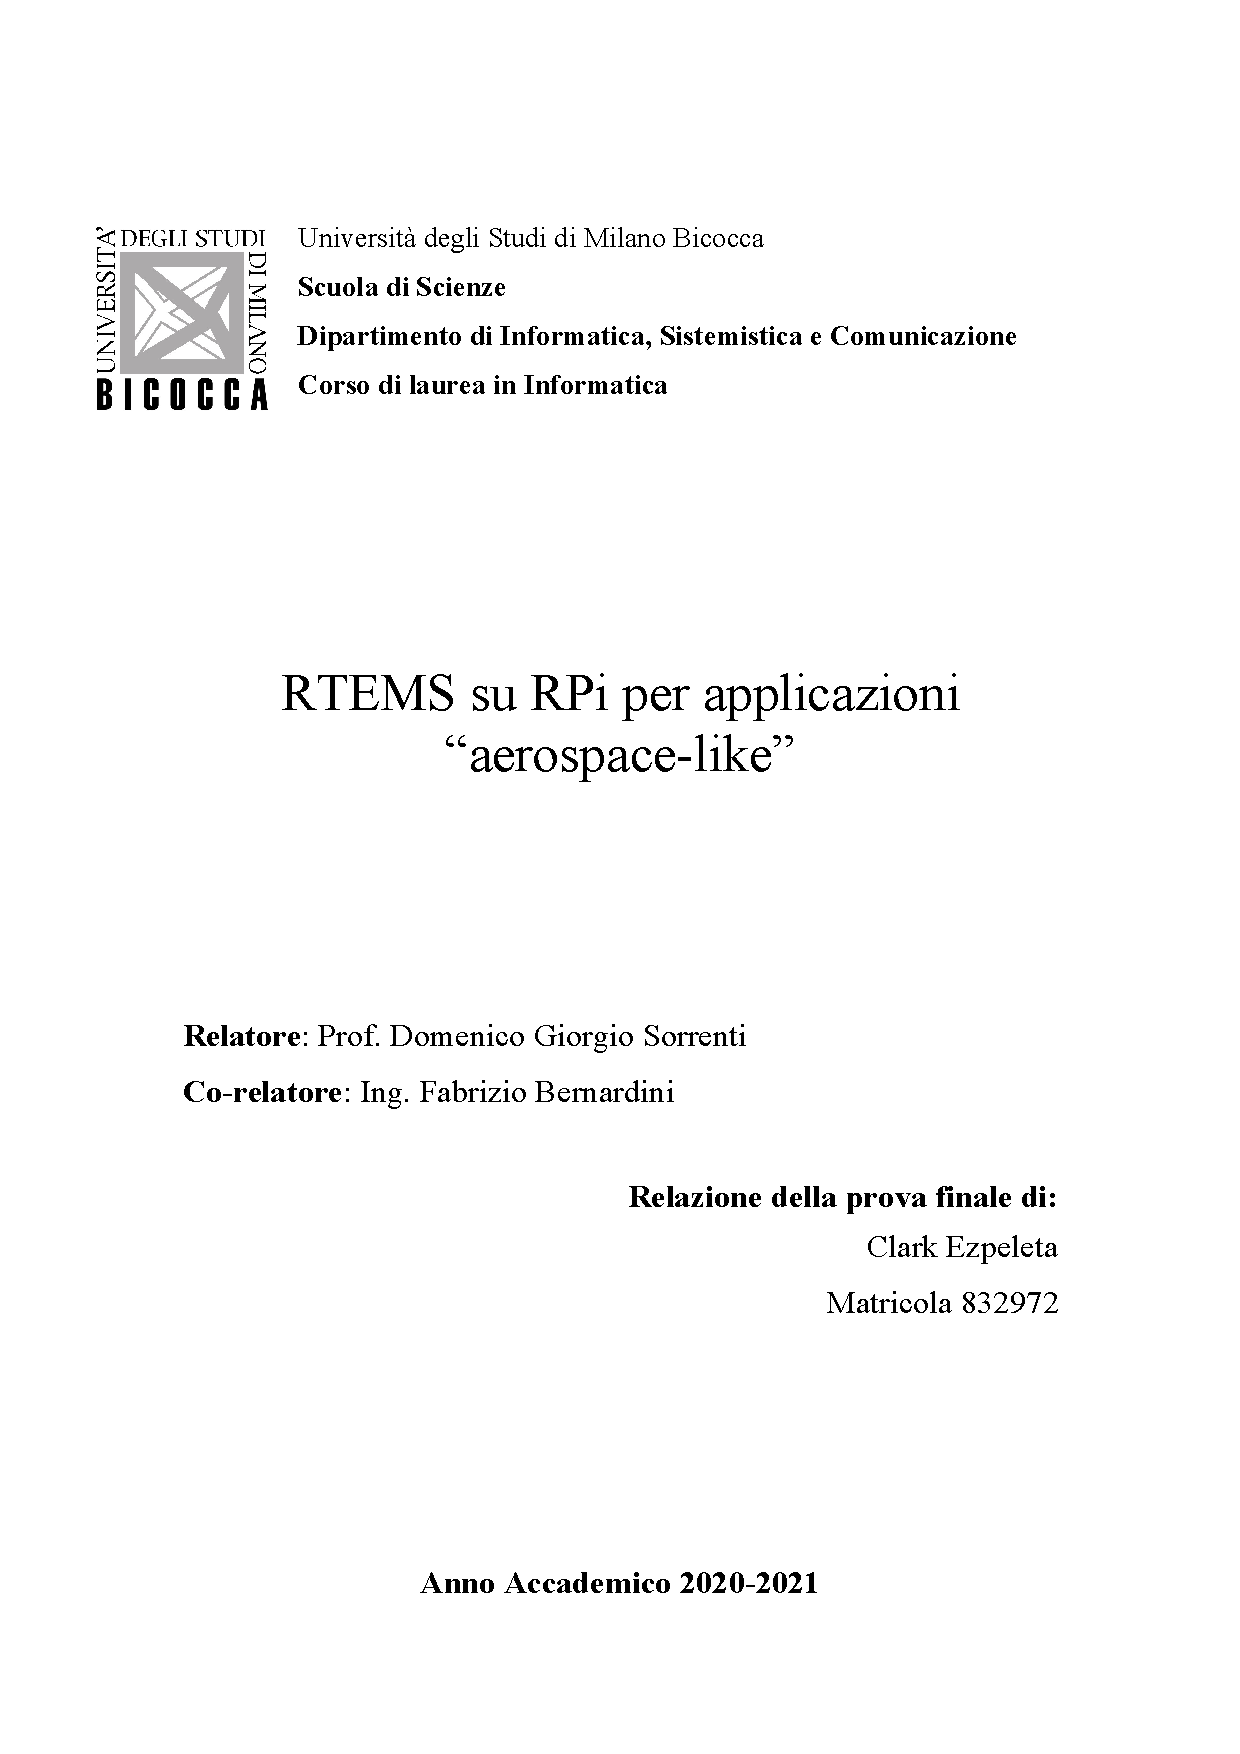
\includepdf[pages={1}]{Frontespizio_Ezpeleta.pdf}
\tableofcontents
\setcounter{page}{0}
\begin{flushleft}
\chapter*{Introduzione}
\setcounter{page}{1}

\addcontentsline{toc}{chapter}{Introduzione} 
Il lavoro che ho svolto ha due obiettivi principali: il 'porting' di RTEMS su Raspberry Pi e la creazione di applicativi RTEMS per validare il corretto funzionamento delle interfacce GPIO, UART, I2C, SPI  e l'utilizzo degli interrupts tramite le API di RTEMS.\\
%Lo scopo del mio lavoro consiste nel porting di RTEMS su Raspberry Pi e nella creazione di applicativi RTEMS  per testare il funzionamento delle interfacce GPIO, UART, I2C, SPI e l'utilizzo degli interrupts.

Per poter svolgere il 'porting' ho fatto riferimento al RTEMS User Manual\cite{rtemsUM}, per comprendere meglio i concetti di RSB(RTEMS Source Builder) e BSP (board support packages), 
ed ho utilizzato la guida fornita da ing. Basile \cite{giorgio}, di BIS-Italia, che raccoglie tutti i passaggi esposti sul blog di Alan Tech per il porting della versione 4.11.\\
%ed ho utilizzato la guida fornita da AlanC trovata sul suo blog \cite{alanT} in cui viene descritto il porting per la versione 4.11.\\
%Purtroppo la guida non è totalmente corretta, poichè datata a Marzo 2013 ed è stata scritta per la versione di RTEMS precedente a quella che ho utilizzato, cioè la 5.1 che è la più recente e stabile. \\
Purtroppo i passaggi illustrati sul blog non sono totalmente corretti, poichè sono per il porting della versione di RTEMS precedente a quella che ho utilizzato, cioè la 5.1 che è la più recente e stabile.
Il 'porting' puo' essere definito corretto, se alla fine della procedura si riesce a caricare uno degli applicativi di test forniti da RTEMS, su Raspberry Pi senza errori.
%Per questo motivo, dopo esser riuscito a caricare su RPi uno degli applicativi di test, forniti da RTMES, senza errori di compilazione e computazione, mi sono occupato della creazione di 
Dopo aver effettuato correttamente il 'porting', ho creato una guida in italiano  che raggruppa tutti i passaggi effettuati integrando le correzioni necessarie, ed è stata corretta anche la guida di ing. Basile \cite{giorgio5}.\\
Dopo aver impostato l'ambiente di lavoro ho iniziato a creare gli applicativi RTEMS da eseguire sulla Raspberry Pi.\\
Per poter creare gli applicativi RTEMS ho dovuto  familiarizzare con il linguaggio C, leggere l'RTEMS Classi API Guide \cite{rtemsCAG} ed analizzare i codici sorgente di esempio trovati nel git repository di asuol\cite{asuol} per poter compredere l'utilizzo delle API. \\
Tutto il lavoro è stato eseguito in modalità "smart-working", per questo motivo mi è stata messa a disposizione da BIS-Italia la scheda Raspberry Pi 3B+ per poter effettuare l'attività.Microchip Technologies ha gentilmente offerto dei componenti aggiuntivi utili per gli applicativi RTEMS di test dell'interfaccia I2C e SPI.\\
Oltre all'attività software ho dovuto eseguire una piccola attività hardware, cioè creare dei circuiti saldando i vari componenti e utilizzando la breadboard in modo da poterli collegare alla Raspberry Pi, per fare ciò ho seguito gli schemi elettrici che mi ha inviato ing. Bernardini e ho letto i datasheet dei componenti dell'interfaccia I2C \cite{microchipMCP3425} \cite{microchipADC} e  SPI \cite{microchipMCP4822} \cite{microchipMSOP10-8} in modo da comprendere il loro funzionamento e poter creare i driver.\\
%Con il materiale ricevuto ho costruito, grazie agli schemi elettrici che mi ha inviato Fabrizio Bernardini, dei circuiti saldando i vari componenti ed utilizzando la breadboard in modo da poterli collegare alla Raspberry Pi.
%Oltre agli schemi elettrici ho letto i datasheet dei componenti I2C \cite{microchipMCP3425} \cite{microchipADC} e  SPI \cite{microchipMCP4822} \cite{microchipMSOP10-8} ricevuti dalla Microchip, in modo da comprendere il loro funzionamento e creare i driver.
%%Grazie all'aiuto di Fabrizio Bernardini sono riuscito a creare i circuiti elettrici su cui far girare i programmi
Premesso tutto ciò ho suddiviso la mia relazione nei seguenti capitoli:

\begin{itemize}
    \item \textbf{Capitolo 1} - in questo capitolo vengono descritte le principali tecnologie utilizzate durante il mio lavoro. Innanzitutto viene descritto RTEMS che è il sistema operativo su cui si basa tutta l'attività, dopodichè viene  descritta la Raspberry Pi su cui verranno eseguiti gli applicativi RTEMS, ed infine viene descritto Eclipse che è l'IDE utilizzato per creare gli applicativi.
    \item \textbf{Capitolo 2} - in questo capitolo viene descritta tutta l'attività di porting e la definizione della toolchain per poter realizzare applicativi RTEMS. Vengono esposte tutte le problematiche rilevate e le loro soluzioni. 
    \item \textbf{Capitolo 3} - in questo capitolo vengono descritti le API che RTEMS ha a disposizione, la loro struttura e in che modo li ho testati e per quali motivi si è scelto di testarli.
    \item \textbf{Capitolo 4} - in questo capitolo viene descritta l'attività software che si basa sulla creazione degli applicativi RTEMS per testare il corretto funzionamento delle API di RTEMS. Viene esposto anche una descrizione dei componenti aggiuntivi offerti da Microchip di cui ho creato i driver per poterli utilizzare con RTEMS.
    \item \textbf{Capitolo 5} - in questo capitolo viene descritto ciò che si è raggiunto e la possibile estensione del mio lavoro.
\end{itemize} 
\chapter{Tecnologie}

\section{RTEMS}
\begin{figure}[h]
    \centering
    
\includegraphics[scale = 2]{rtemslogo.png}
\end{figure}
RTEMS sta per Real-Time Executive MultiProcessor System ed è un sistema operativo real-time (RTOS) general purpose open source (licenza GPL 2.0 modificata) progettato e gestito da OAR Corporation. Il suo sviluppo iniziò nella fine degli anni 80 utilizzando i linguaggi Ada e C, e venne usato inizialmente per scopi militari, invece le prime versioni utilizzabili sono state rese open-souce su server ftp nel 1994.\\
Attualmente viene utilizzato in molti settori tra cui quello aereospaziale, infatti è stato utilizzato in alcune missioni spaziali sia a livello di on-board computer che come computer embedded in altre attività di volo
%ad esempio sul MRO (Mars Reconnaissance Orbiter) è in esecuzione un applicativo RTEMS che controlla l' Electra UHT Transceiver (EUT) che serve per la comunicazione tra Marte e la Terra . \\
RTEMS è  stato validato dall'ESA, European Space Agency, ciò vuol dire che sono stati scritti dei programmi che riproducono gli scenari critici (ad esempio la gestione di molti device oppure la gestione e l'esecuzione concorrente dei task), e sono stati eseguiti sul sistema operativo per poter verificare il suo corretto funzionamento in quei casi. La validazione viene tutt'ora aggiornata poiché è un sistema operativo che è in continua evoluzione e avrà più funzionalità con il passare del tempo.\\
RTEMS non è un sistema operativo a sé stante, usato epr caricare altri programmi, ma è un executive che viene compilato con l'applicaizone in un unico codice monolitico da eseguire.
%RTEMS è un Real-Time Executive ciò vuol dire che si possono creare applicativi RTEMS che fanno da kernel alla macchina su cui vengono eseguiti. Gli applicativi prendono il controllo su tutto la scheda.\\
%Un real-time multitasking executive è un applicativo che è formato da un insieme di task indipendenti tra di loro.Ogni task sono internamente sincroni, ma diversi tasks possono essere eseguiti indipendentemente, risultando un processo asincrono nell insieme.
\newpage
RTEMS puo' essere visto come un insieme di direttive raggruppate in una serie di manager, che si occupano di varie funzionalità tra cui il controllo e la sincronizzazione dei task e processori, la gestione della memoria e la mutua esclusione. Invece la gestione dello scheduling, dispatching e object management sono forniti dal executive core.
\begin{figure} [h]
    \centering
    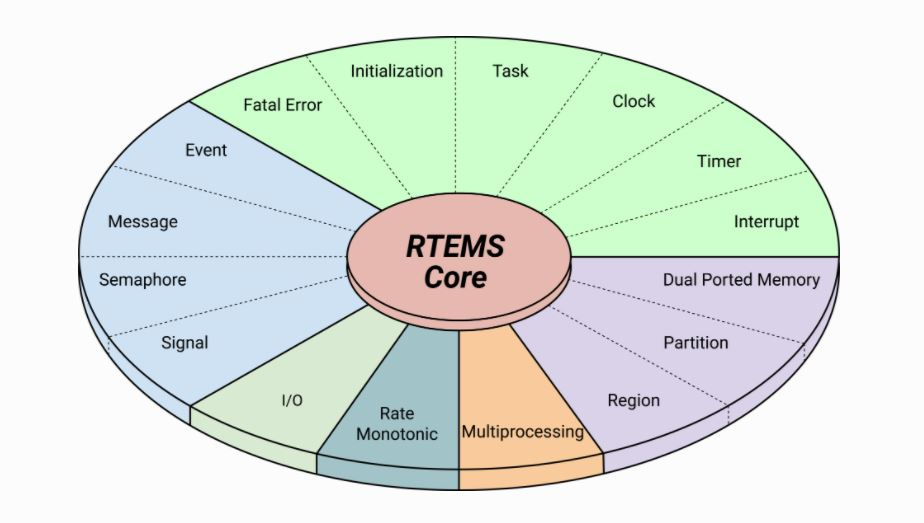
\includegraphics[scale = 0.80]{rtems_internal_architecture.JPG}
    \caption{Architettura RTEMS}
    \label{fig:my_label1}
\end{figure}

Utilizzando i managers di RTEMS lo sviluppatore puo' concentrarsi al solo sviluppo del applicativo e ciò riduce notevolmente il tempo di sviluppo.\\

La figura successiva mostra la logica di utilizzo di RTEMS.
\begin{figure}[ht]
    \centering
    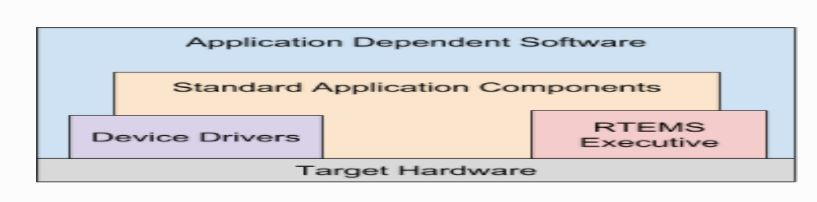
\includegraphics[scale = 0.80]{application_architecture.JPG}
    \caption{Struttura applicativo RTEMS}
    \label{fig:my_label2}
\end{figure}

Come si puo' notare RTEMS Executive è un intermediario tra il codice dell'applicativo e il target hardware, invece le dipendenze hardware con altri device sono localizzati nel livello "device drivers".
Il RTEMS I/O manager incorpora queste dipendenze hardware nel sistema mentre allo stesso momento fornisce all'application code l'accesso ad esse.
Queste dipendenze hardware sono isolate in specifiche BSP, Board Support Packages, per questo motivo il porting di un applicativo RTMES su altri processori è semplice poichè basterebbe selezionare la BSP del microprocessore su cui si vuol eseguire l'applicativo e compilare con le sue librerie.\\
In questo modo durante lo sviluppo di un applicativo real-time si ha la totale indipendenza dall'architettura dei microprocessori. \\

E' disponibile il porting di RTEMS su molte architetture CPU tra cui ARM, MIPS, LEON,ERC32 e i PowerPC; durante il mio lavoro ho trattato il porting su architettura ARM utilizzando una Raspberry Pi 3B+.
\section{Raspberry Pi}
\begin{figure}[h]
    \centering
    
\includegraphics[scale = 0.70]{raspberrypiLogo.png}
\end{figure}
Raspberry Pi è una serie di computer a scheda singola sviluppata da Rasberry Pi Foundation in collaborazione con la Broadcom, in Inghiterra.\\
Originariamente è stato usato per insegnare le basi dell'informatica nelle scuole e nei paesi in via di sviluppo, ma attualmente grazie al suo basso prezzo viene usato anche nel settore della robotica, domotica e in molti altri.
Al momento sono state rilasciate quattro generazioni di Raspberry Pi, e tutti i modelli hanno un Broadcom SoC (System on Chip) con processore ARM integrato e on-chip GPU (Graphics Processing Unit).\\
Durante il mio lavoro viene usata la \textbf{Raspberry Pi 3B+} che utilizza il Broadcom BCM2837B0 SoC \cite{bcm2837} con processore Cortex-A53 (ARMv8) 64-bit 1.4GHz.
\newpage
\begin{figure} [h]
    \centering
    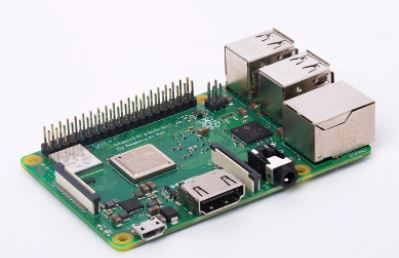
\includegraphics[scale = 1.25]{RPi3B.JPG}
    \caption{Scheda Raspberry Pi 3B+}
    \label{fig:RPI3B_laver}
\end{figure}
Tra le specifiche tecniche quelle che ci interessano maggiormente sono:
\begin{itemize}
    \item SDRAM LPDDR2 da 1GB.
    \item supporto per la micro SD.
    \item accesso a 40 GPIO.
\end{itemize}

La memoria micro SD viene utilizzata per il caricamento degli eseguibili RTEMS nel seguente modo:
\begin{enumerate}
    \item viene copiato il firmware di Raspberry Pi compatibile con RTEMS nella memoria SD.
    \item bisogna cancellare i file 'kernel*.img'. 
    \item compilare i sorgenti di un applicativo RTEMS in modo da ottenere il file con estensione'.img' 
    \item copiare l'eseguibile RTEMS nella memoria SD.
    \item impostare l'eseguibile RTEMS come kernel della scheda Raspberry Pi, modificando il file 'config.txt'
\end{enumerate}
In questo modo all'accensione della Raspberry Pi, l'eseguibile è il kernel della scheda e viene eseguito automaticamente.

\newpage
La figura successiva mostra tutti i pin GPIO che Raspberry Pi 3B+ ha a disposizione:
\begin{figure}[h]
    \centering
    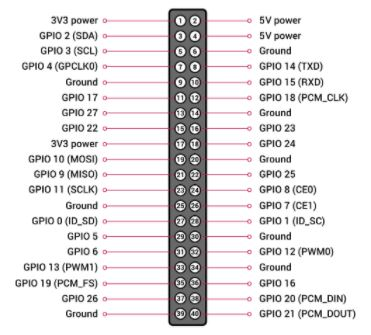
\includegraphics[scale = 1.50]{RPi3B_GPIO.JPG}
    \caption{Raspberry Pi 3B+ GPIO}
    \label{fig:RPi3B_GPIO}
\end{figure}

Tutti i pin configurabili hanno un output da 0v a 3v3 e come input sono 3v3 'tollerant'.

%TODO :  forse da aggiungere più descrizione GPIO

\newpage

\section{Eclipse}
Eclipse è un IDE open source rilasciato con licenza EPL (Eclipse Public License) creato da IBM usato principalmente per la programmazione in Java ma grazie a vari plugin puo' essere usato per altri linguaggi di programmazione come C, C++, COBOL, Python e molti altri. \\
L'ambiente di sviluppo Eclipse include l'Eclipse Java development tools per Java, e l'Eclipse CDT per C/C++. \\
Per utilizzare RTEMS gcc cross compiler su Eclipse C, bisogna installare il plugin di RTEMS e settare le variabili di ambiente.
%TODO : aggiungere schermata con uno dei programmi che ho fatto
\chapter{Porting di RTEMS su RPi}
%Qui ci va sia l'attività di porting (download, versioni, organizzazione) fino alla prima prova, ed anche la definizione della "toolchain" per programmare in C e realizzare applicazioni RTEMS.


L'attività di porting è la prima fase del lavoro e consiste in:
\begin{enumerate}
    \item Installazione dalla tool-suite sul computer host, dove vengono creati gli applicativi RTEMS.
    \item Verifica del corretto funzionamento della tool-suite, eseguendo i programmi di test su Raspberry Pi
    \item Configurazione del IDE Eclipse C, per la creazione di eseguibili RTEMS
    \item Provare a compilare e eseguire i programmi sia da terminale, e sia da Eclipse C
\end{enumerate}
Per svolgere tutta la procedura mi sono munito di un computer con sistema operativo Ubuntu, una scheda Raspberry Pi 3B+, una microsd, e convertitore TTL USB.\\
%Tutta la procedura viene effettuata tramite comandi eseguiti su terminale.

%Per poter eseguire l'attività è necessario avere un computer con sistema operativo Ubuntu 
%(si potrebbe usare anche Windows o IOs ma con Ubuntu il procedimento è più semplice),
%una scheda Raspberry Pi .\\
RTEMS in sé è complesso per questo il team di RTEMS ci fornisce "l'ecosistema di RTEMS" che è una collezione di strumenti, packages, codici sorgente e documentazione, utile per definire come sviluppare, mantenere e usare RTEMS.\\
Durante il porting ho utilizzato due importanti strumenti che fanno parte dell'ecosistema RTEMS, e sono :
\begin{itemize}
    \item RTEMS RSB = l'RTEMS Source Builder è tool molto utile per compilare e buildare i moduli di RTEMS e delle BSP 
    \item BSP  raspberrypi = la Build Support Package è il codice di supporto, che contiene le librerie di RTEMS per una specifica scheda (ad esempio la BSP raspberrypi viene usata per la Raspberry Pi 3B+)
\end{itemize}
Dopo aver effettuato correttamente tutti i passaggi per il porting, ho creato una guida che li espone, in questo modo che qualunque utente voglia approcciarsi ad RTEMS su RPi per la prima volta riesca ad eseguirlo senza dover cercare tra le tante fonti sparse su internet.

%TODO da capire se mettere come indice la guida del porting oppure nelle conclusioni con un elenco dei "prodotti" realizzati
\chapter{Integrazione hardware e software}
%Qui ci va una descrizione delle varie interfacce disponibili in termini di drivers SW e come le abbiamo provate.

%RTEMS ha vari driver disponibili per l'utilizzo delle interfacce hardware
Effettuato il porting sono passato all'attività software, cioè la creazione di RTEMS executive per testare il funzionamento delle RTEMS Classic API che sono le API per l'utilizzo delle interfacce. \\
\begin{figure} [h]
\centering
    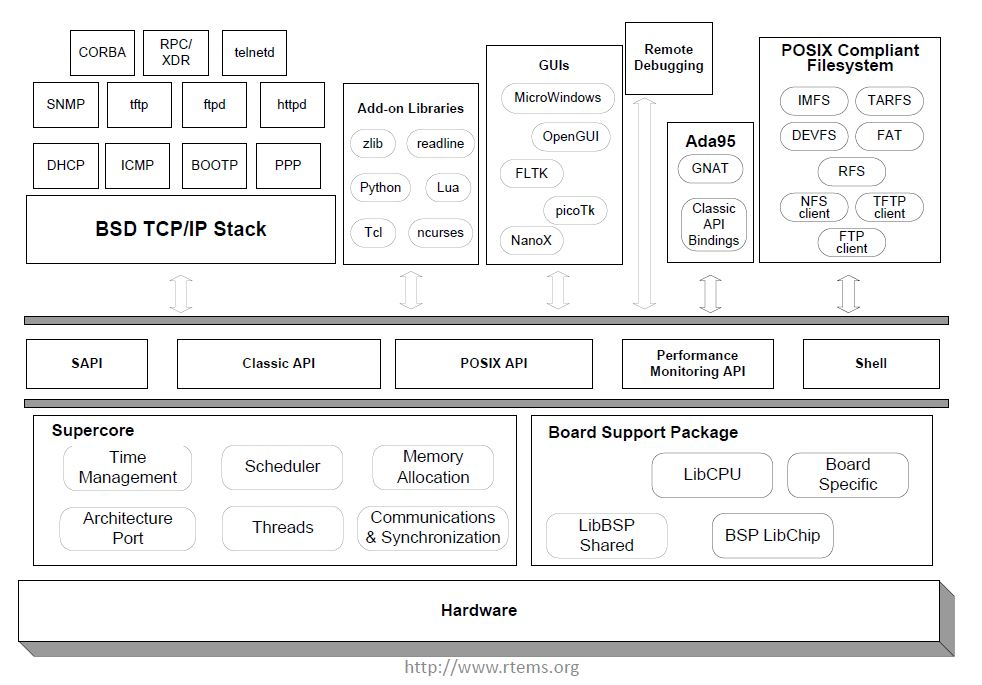
\includegraphics[scale = 0.80] {RTEMS_architecture.JPG}
    \caption{Architettura dettagliata sistema RTEMS}
    \label{fig:my_label3}
\end{figure}
%TODO elenco delle interfacce e api che ci interessano
Le interfacce che ci interessano validare sono:
\begin{itemize}
    \item UART
    \item GPIO
    \item I2C
    \item SPI
\end{itemize}

%Le interfacce che ho testato sono ;
---\\
TODO\\
----\\
%Con l'attività di porting si è potuto verificare il funzionamento dell'interfaccia UART, come porta per i log di sistema che verranno utilizzati durante il debug degli applicativi RTEMS.

\chapter{Attività sperimentale}
\section{Obiettivi}
%Nell'ambito dei sistemi embedded, e soprattutto nel settore spaziale, il risultato del software oltre al'esito computazionale dipende anche dal 
Gli obiettivi dell'attività sperimentale sono:

TODO
%  Requisiti di validazione: cosa vogliamo provare, come e perchè. Ci sono degli agganci al mondo spaziale qui.

\section{Test set-up}
%Descrizione del sistema in generale e della/e scheda/e aggiuntiva/e per fare i vari test dell'HW
Ogni programma di test creato implica un circuito elettrico differente costruito con jumper, breadboard, resistenze, condensatori, pulsanti, LED e schede aggiuntive mandate dalla Microchip su cui ho dovuto saldare cavetti e componenti per poterli utilizzare e collegare alla Raspberry Pi.\\

I componenti aggiuntivi sono :
\begin{itemize}
    \item MCP3425 SOT23-6 Evaluation Board  \cite{microchipMCP3425}: un evaluation board, con un ADC (Analog Digital Converter) MCP3425, controllato tramite protocollo I2C
    \item MSOP-10 and MSOP-8 Evaluation Board \cite{microchipMSOP10-8}: un evaluation board generica che serve per il collegamento del componente MCP4822 alla Raspberry Pi
    \item MCP4822 \cite{microchipMCP4822}: un DAC (Digital Analog Converter) controllato tramite protocollo SPI, montato sulla evaluation board sopracitata.
\end{itemize}
\newpage
Il componente MPC3425 è un ADC da 16 bit che ha come input due tensioni $V_{IN}^+ $ e $ V_{IN}^-$ e come output una tensione pari a $V_{IN}^+ - V_{IN}^- \times PGA$. Il componente ha la seguente configurazione predefinita:
\begin{itemize}
    \item Programmable Gain Amplifier(PGA) = 1
    \item Continuos Conversion
    \item Programmable Data Rate = 12 bit
\end{itemize}
Durante il lavoro viene utilizzata questa configurazione, ma nel caso si volesse cambiare la configurazione del componente, si puo' eseguire una scrittura di due byte dove il primo byte rappresenta l'indirizzo di periferica e il bit R/W (nel nostro caso è 11010000) invece il secondo contiene i bit di configurazione\\
\begin{figure}[h]
    \centering
    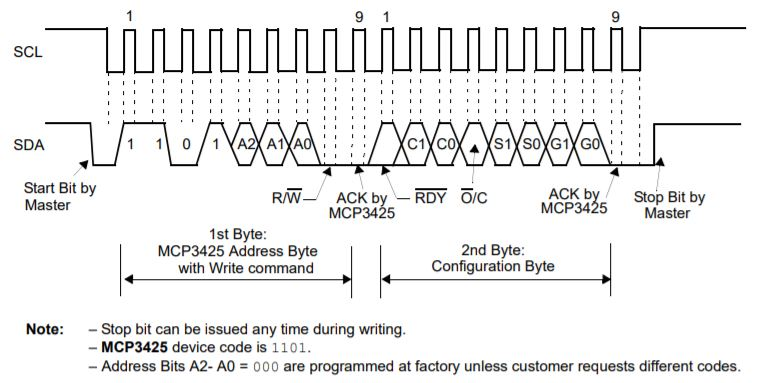
\includegraphics{wrtie_configuration_MCP3425.JPG}
    \caption{Diagramma temporale scrittura su MCP3425}
    \label{fig:my_label4}
\end{figure}
La lettura del valore in uscita dal DAC deve essere eseguita nel seguente modo:
\begin{enumerate}
    \item mandare sul bus I2C l'indirizzo di periferica con R/W pari a 1
    \item lettura dei due byte
    \item conversione dei byte per avere il valore effettivo della tensione
\end{enumerate}
---\\
TODO : DESCRIZIONE COMPONENTE MCP4822\\
---\\
TODO: DESCRIZIONE CIRCUITI\\
---\\
\section{Test application software}
La struttura principale che tutti i programmi seguono è la seguente:
\begin{itemize}
    \item init.c = è il file sorgente contenente la funzione Init che è il punto di partenza dell'eseguibile. E' come se fosse il metodo main in Java.
    \item init.h = è un file header che contiene tutte le direttive RTEMS per configurare il sistema
    \item task\_helper.c = è il file sorgente contenente la definizione dei task, le funzioni per la manipolazione delle variabili globali, le funzioni aggiuntive 
    \item task\_helper.h = è un file header che contiente tutte le dichiarazioni delle funzioni definite in task\_helper.c che si vogliono usare in init.c, ad esempio la definizione dei task.
\end{itemize}

%Architettura del programma di prova di un po' tutto
Il programma di test del UART si tratta di un semplice "hello world!" è stato il più semplice da creare, poichè durante il porting è stato usato un programma di esempio simile per visualizzare i log di sistema. Dal codice sorgente dei programmi di esempio, come quelli per il ticker.img,  si puo' ipotizzare correttamente che per far stampare un messaggio sulla console è sufficiente definire la direttiva di sistema 
\begin{lstlisting}
#define CONFIGURE_APPLICATION_NEEDS_SIMPLE_CONSOLE_DRIVER 
\end{lstlisting} 
e usare le funzioni della libreria standard stdio.h 
\begin{lstlisting}
printf("log"); 
fflush(stdout);
\end{lstlisting}
L'interfaccia GPIO è stata testata con tre programmi per coprire le seguenti situazioni :
\begin{itemize}
    \item accensione e spegnimento di un led ad intervalli di 1 secondo.
    \item alla pressione di un bottone si ha l'accesione o spegnimento di un led.
    \item alla pressione di un bottone, viene avviato un task.
\end{itemize}
---\\
TODO : DESCRIZIONE DEL PRIMO PROGRAMMA\\
---\\
TODO: DESCRIZIONE DEL SECONDO PROGRAMMA, DESCRIVENDO COME è STATA GESTITA LA SEZIONE CRITICA\\
---\\
TODO: DESCRIZIONE DEL TERZO PROGRAMMA, DESCRIVENDO LA GESTIONE DEI TASK CON INTERRUPT\\
---\\
L'interfaccia I2C è stata testata creando un programma che legge dal SDA l'output del componente ADC che manipolandolo come indicato dal datasheet mi da come risultato la tensione in entrata al ADC. Poichè bisogna utilizzare un componente aggiuntivo, ho dovuto creare il driver associato.\\
---\\
TODO : DESCRIZIONE PROGRAMMA I2C E DEL DRIVER\\
---\\
Per testare l'interfaccia SPI è stato creato un programma che legge dal MOSI l'output del componente che dovrebbe rappresentare la tensione in uscita. Anche in questo caso si è dovuto creare il driver associato \\
---\\
TODO : DESCRIZIONE PROGRAMMA SPI E DEL DRIVER\\
---\\
\section{Risultati finali}
TODO\\
	%Risultati delle prove fatte, problemi riscontrati, etc.Un po' una descrizione del lavoro svolto per dimostrare che quello che è specificato nel cap 5 è stato fatto davvero. Qui aiutano anche dati presi con la strumentazione, se possibile.
\chapter{Conclusioni}
TODO\\
----\\
%Nel capitolo 1 ti sei dato degli obiettivi e qui devi dimostrare che li hai raggiunti.

Il lavoro svolto fa parte dei progetti di BIS-Italia, sezione italiana della British Interplanetary Society, società storica britannica di cui sono membro, che mi ha seguito durante lo stage. BIS-Italia prevede di utilizzare RTEMS su RPi per il progetto di una replica in scala 1:3 di ExoMars Rover che verrà utilizzato per divulgazione.\\
Tutto il lavoro è stato svolto con l'aiuto dei membri di BIS-Italia e la collaborazione di Microchip.
\chapter*{Ringraziamenti}
\printbibliography
\end{flushleft}

\end{document}
